\documentclass[fleqn,10pt]{wlscirep}
\usepackage[utf8]{inputenc}
\usepackage[T1]{fontenc}
\title{Brain Lateralization in Alzheimer's Disease}

\author[1]{Yile Wang}
\author[1,*]{Ana Solodkin}
% \author[1,2,+]{Christine Author}
% \author[2,+]{Derek Author}
\affil[1]{Department of Neuroscience, School of Behavioral and Brain Science, The University of Texas at Dallas, Richardson, 75080, USA}
% \affil[2]{Affiliation, department, city, postcode, country}

\affil[*]{email: solodkin@utdallas.edu}

% \affil[+]{these authors contributed equally to this work}

\keywords{Lateralization, Alzheimer's Disease, TheVirtualBrain}

\begin{abstract}
The alternation of the brain lateralization has been reported from many studies. 
\end{abstract}
\begin{document}

\flushbottom
\maketitle
% * <ylwwayne@gmail.com> 2015-02-09T12:07:31.197Z:
%
%  Click the title above to edit the author information and abstract
%
\thispagestyle{empty}

% \noindent Please note: Abbreviations should be introduced at the first mention in the main text – no abbreviations lists. Suggested structure of main text (not enforced) is provided below.
\setlength{\parindent}{0pt} % 
\section*{Introduction}


Brain Lateralization in healthy aging and AD:

In William Calvin’s book ‘The Throwing Madonna’,  \cite{calvin_throwing_2010} \par
\vspace*{1\baselineskip} 
AD is a disconnection syndrome:
From an early stage of Alzheimer’s Disease (AD) research, scientists have realized that AD pathology is a consequence of disturbance of the brain connectivity \cite{delbeuck_alzheimer_2003}. Till today, a growing volume of literature has demonstrated that Alzheimer’s Disease (AD) is a brain disconnection syndrome \cite{brier_network_2014} \cite{delbeuck_alzheimer_2003} \cite{reid_structural_2013} \cite{stam_graph_2009} from several aspects. Daianu and colleagues have found widespread structural connectivity breakdown in AD patients brain networks compared to normal aging \cite{daianu_breakdown_2013}. From network analysis, almost all the AD studies have reported that some brain network features such as the long range connectivity \cite{stam_magnetoencephalographic_2006}, interhemispheric connectivity \cite{qiu_inter-hemispheric_2016}, node centrality, synchronizability and modularity have decreased in AD \cite{stam_modern_2014}. All the evidence suggests that the disconnection syndrome might be a major manifestation of the progression of the AD.\par
\vspace*{1\baselineskip} 
Decrease of interhemispheric connectivity in AD:
In all range of these disconnection syndromes, decrease of the interhemispheric connectivity is one of the most common results in AD, which has been reported in several studies \cite{daianu_breakdown_2013} \cite{lakmache_interhemispheric_1998} \cite{wang_interhemispheric_2015}. \par



\section*{Results}

Up to three levels of \textbf{subheading} are permitted. Subheadings should not be numbered.\par




\subsection*{Subsection}

Example text under a subsection. Bulleted lists may be used where appropriate, e.g.

\begin{itemize}
\item First item
\item Second item
\end{itemize}

\subsubsection*{Third-level section}
 
Topical subheadings are allowed.

\section*{Discussion}

The Discussion should be succinct and must not contain subheadings.

\section*{Methods}

Topical subheadings are allowed. Authors must ensure that their Methods section includes adequate experimental and characterization data necessary for others in the field to reproduce their work.

\bibliography{sample}

% \noindent LaTeX formats citations and references automatically using the bibliography records in your .bib file, which you can edit via the project menu. Use the cite command for an inline citation, e.g.  \cite{long_distinct_2013}.

% For data citations of datasets uploaded to e.g. \emph{figshare}, please use the \verb|howpublished| option in the bib entry to specify the platform and the link, as in the \verb|Hao:gidmaps:2014| example in the sample bibliography file.

\section*{Acknowledgements (not compulsory)}

Acknowledgements should be brief, and should not include thanks to anonymous referees and editors, or effusive comments. Grant or contribution numbers may be acknowledged.

\section*{Author contributions statement}

Must include all authors, identified by initials, for example:
A.A. conceived the experiment(s),  A.A. and B.A. conducted the experiment(s), C.A. and D.A. analysed the results.  All authors reviewed the manuscript. 

\section*{Additional information}

To include, in this order: \textbf{Accession codes} (where applicable); \textbf{Competing interests} (mandatory statement). 

The corresponding author is responsible for submitting a \href{http://www.nature.com/srep/policies/index.html#competing}{competing interests statement} on behalf of all authors of the paper. This statement must be included in the submitted article file.

\begin{figure}[ht]
\centering
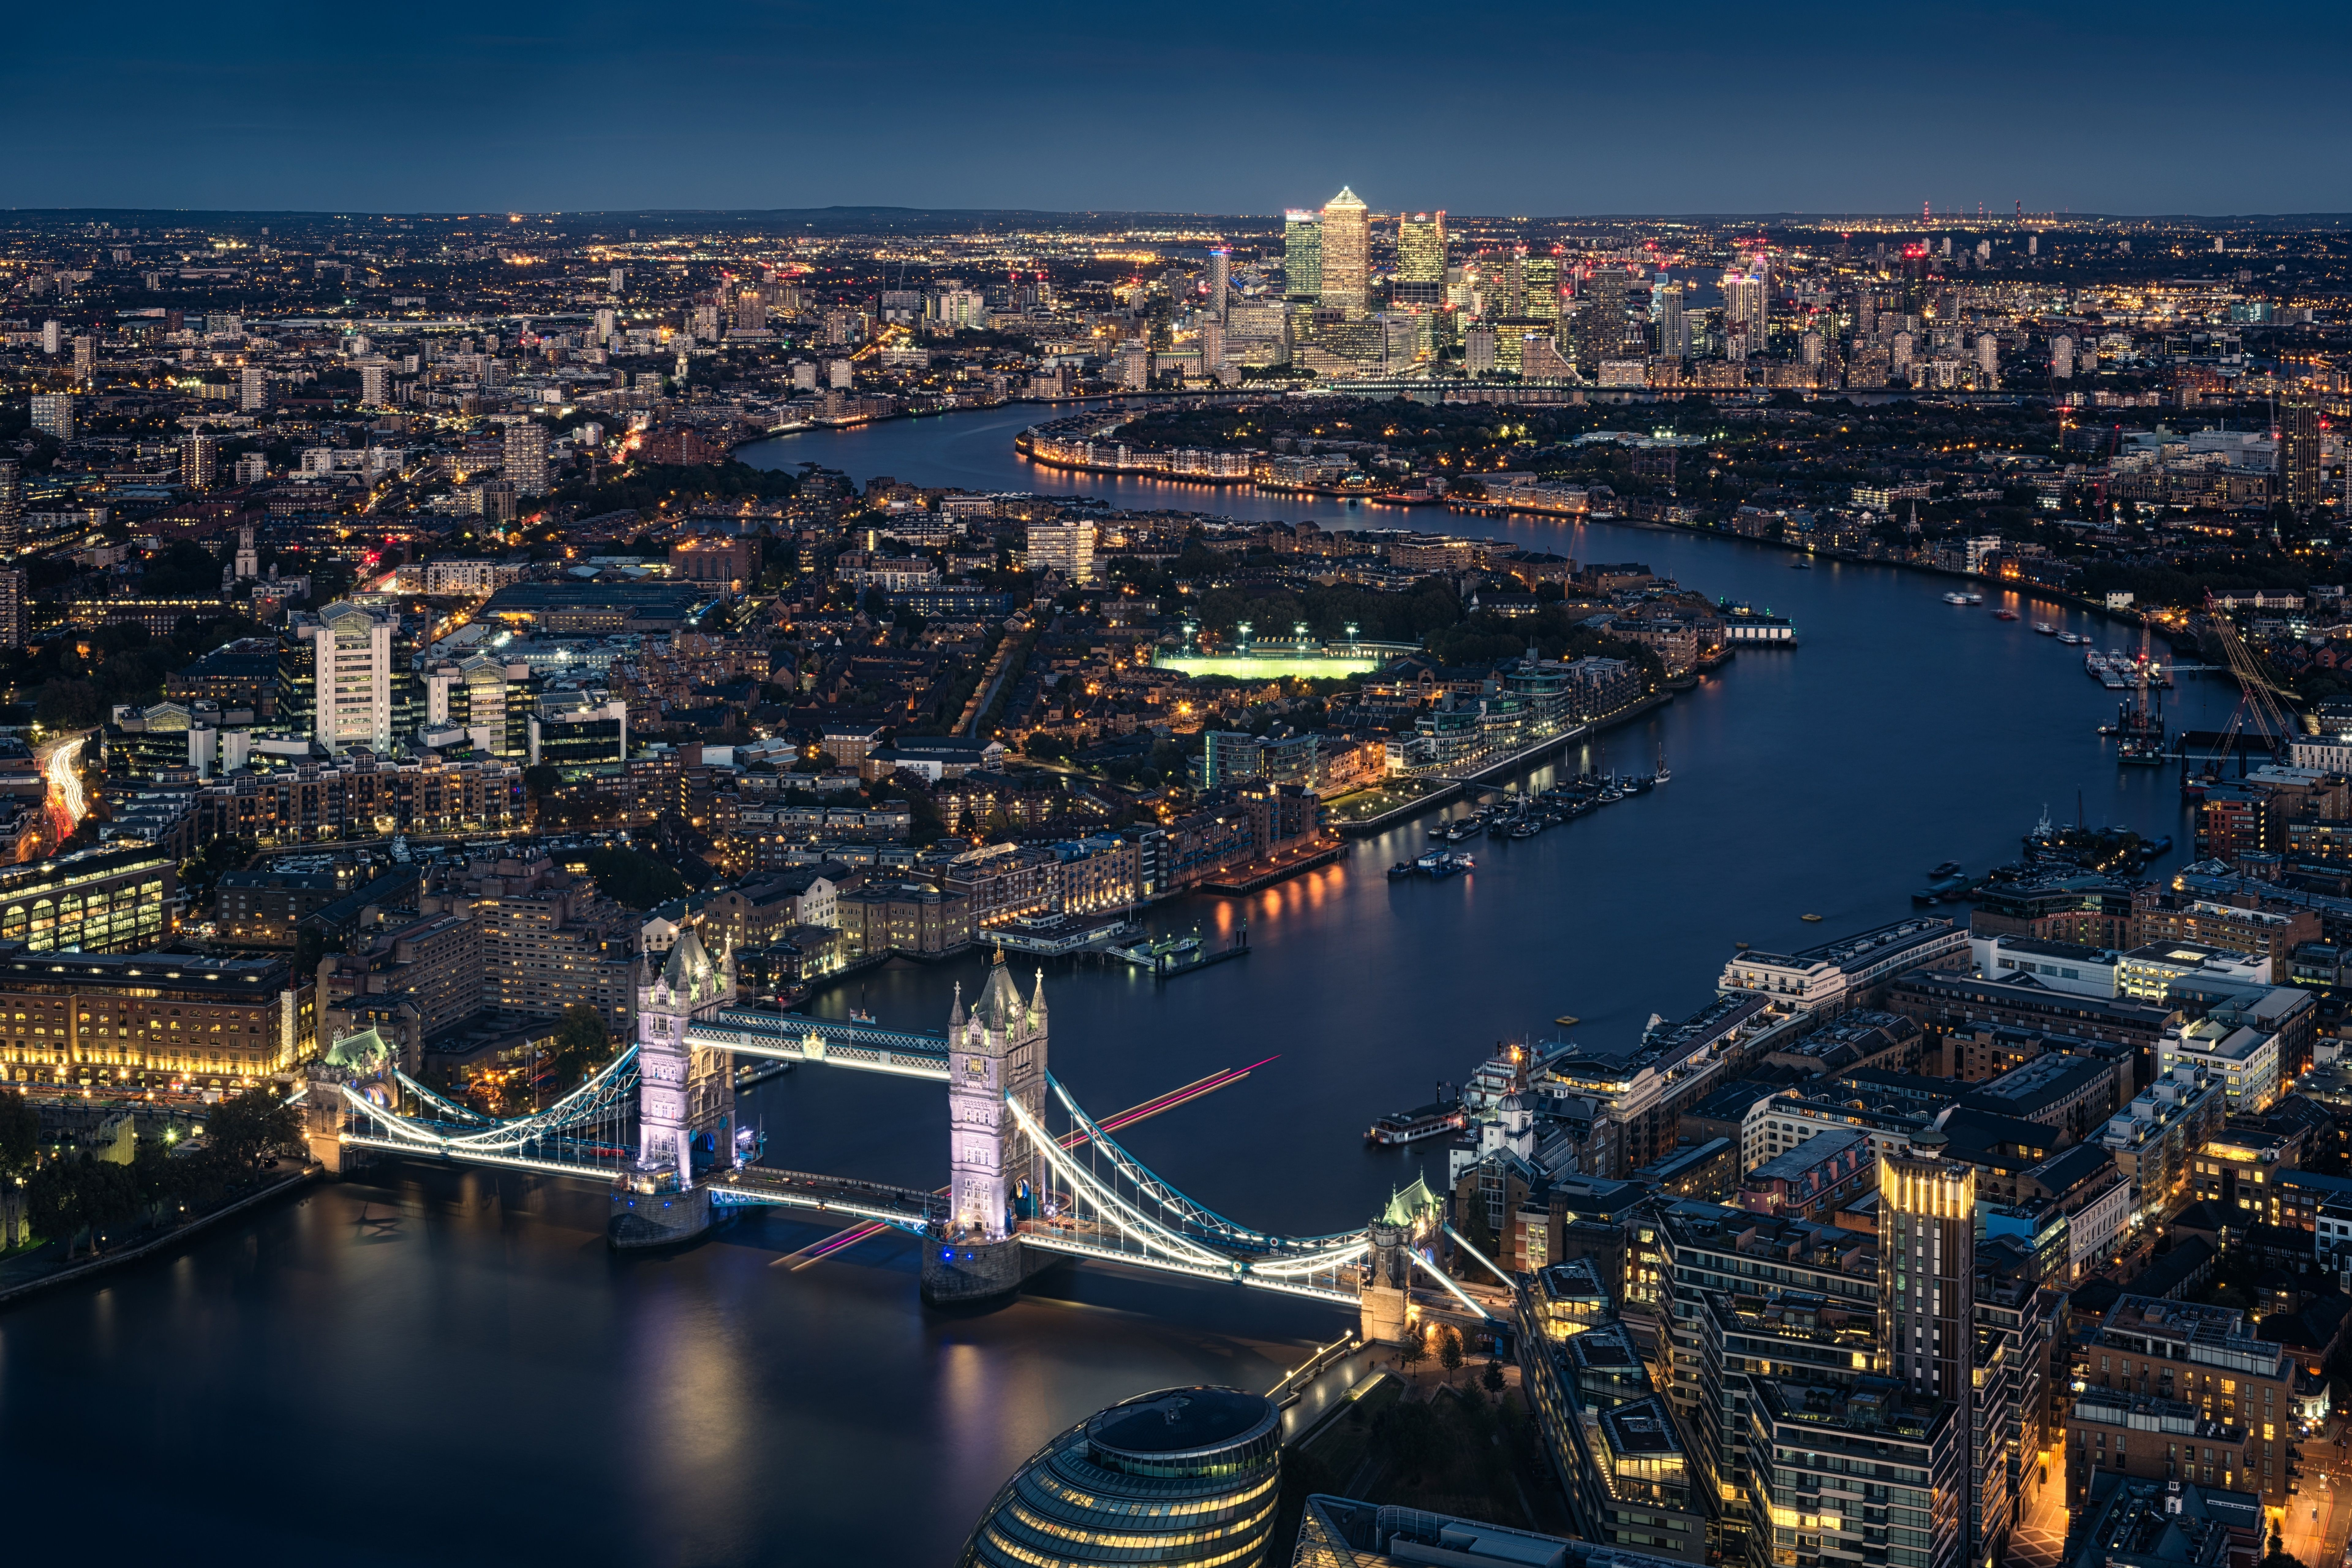
\includegraphics[width=\linewidth]{stream}
\caption{Legend (350 words max). Example legend text.}
\label{fig:stream}
\end{figure}

\begin{table}[ht]
\centering
\begin{tabular}{|l|l|l|}
\hline
Condition & n & p \\
\hline
A & 5 & 0.1 \\
\hline
B & 10 & 0.01 \\
\hline
\end{tabular}
\caption{\label{tab:example}Legend (350 words max). Example legend text.}
\end{table}

Figures and tables can be referenced in LaTeX using the ref command, e.g. Figure \ref{fig:stream} and Table \ref{tab:example}.

\end{document}